\section{Anexos}
\subsection{Repositorio en GitHub}
El desarrollo del proyecto se encuentra en la siguiente dirección: \url{https://github.com/jrsnzc/biblioteca}.

\subsection{Instalación y ejecución de Oracle APEX}
Iniciamos la máquina virtual con el comando \lstinline$vagrant up$.
\begin{figure}[H]
  \centering
  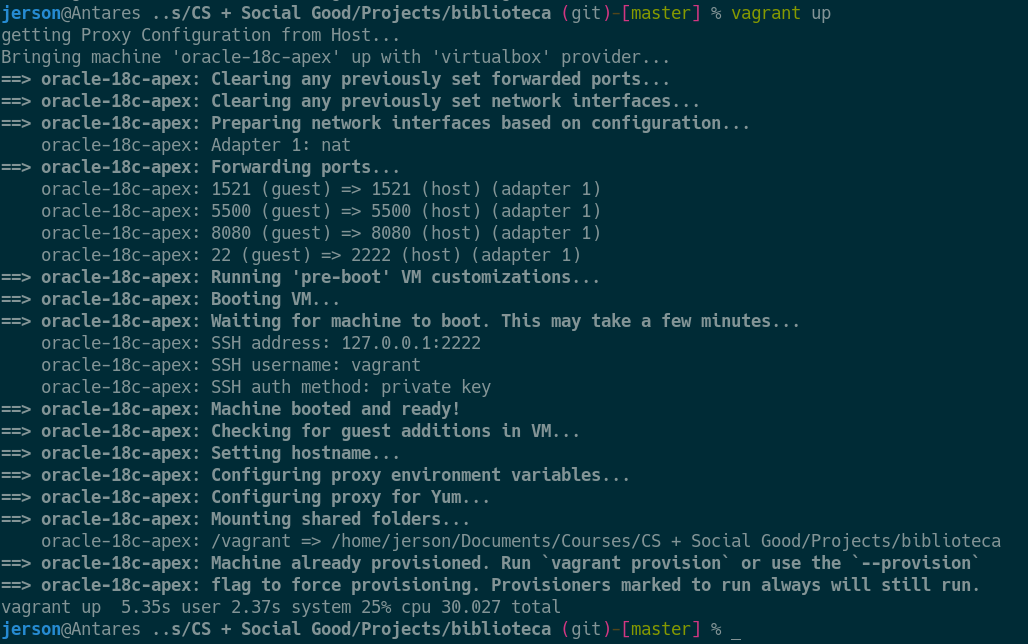
\includegraphics[width=0.9\textwidth]{Vagrant-APEX}
  \caption{Levantamiento de procesos de la máquina virtual} 
  \label{fig:vagrant-apex}
\end{figure}

Creamos una nueva estación de trabajo y un usuario administrador.
\begin{figure}[H]
  \centering
  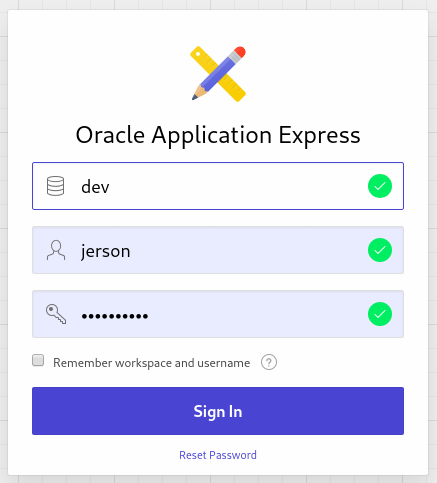
\includegraphics[width=0.9\textwidth]{APEX-login}
  \caption{Oracle APEX, pantalla de inicio de sesión}
  \label{fig:apex-login}
\end{figure}

\subsection{Programa: Sistema de gestión de biblioteca}
\subsubsection{Formularios}
En la figura \ref{fig:biblio-form_libro} se muestra los datos a llenar al crear un nuevo libro. Se elije a que editorial y categoría pertenece.
\begin{figure}[H]
  \centering
  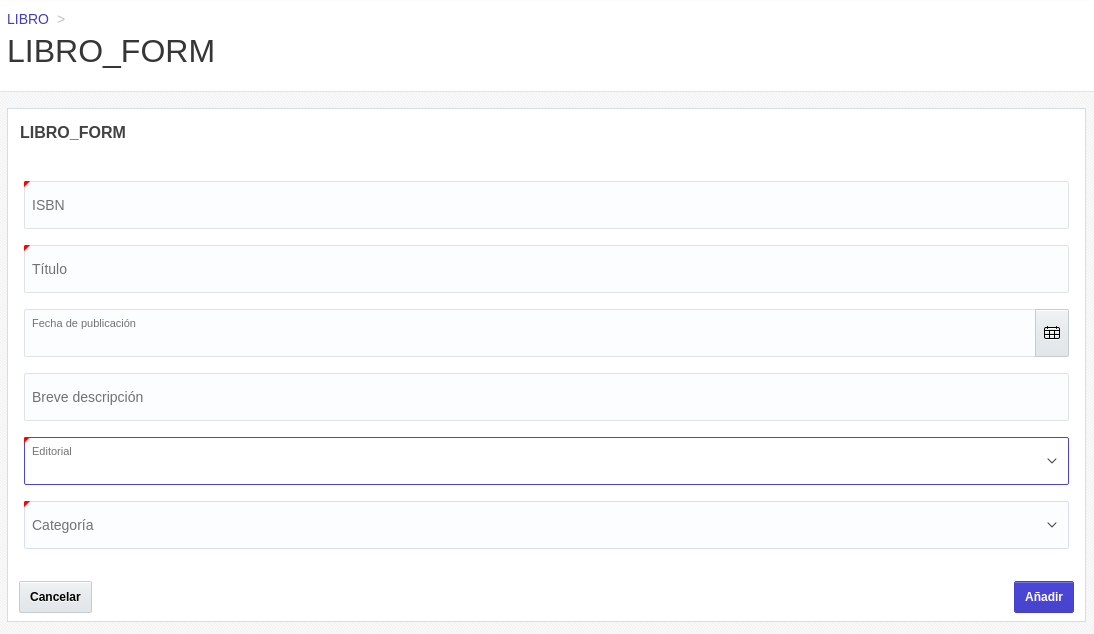
\includegraphics[width=0.95\textwidth]{biblio-form_libro}
  \caption{Formulario para la creación de libros}
  \label{fig:biblio-form_libro}
\end{figure}
\subsubsection{Reportes}
En la figura \ref{fig:biblio-report_libro} se muestra los libros con los que cuenta la biblioteca.
\begin{figure}[H]
  \centering
  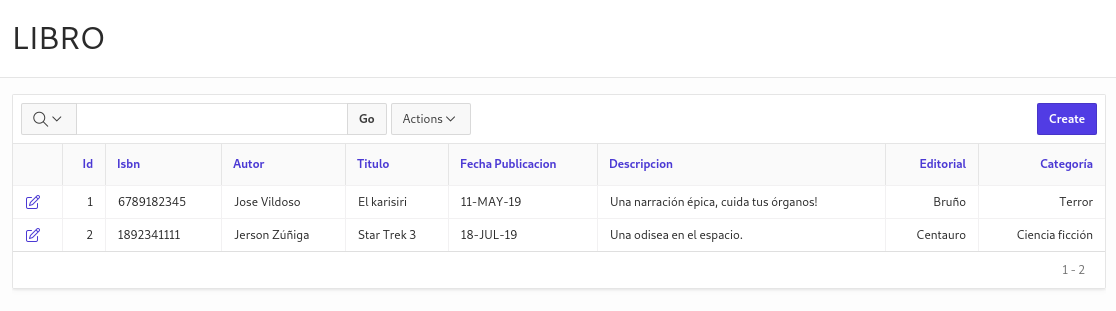
\includegraphics[width=0.95\textwidth]{biblio-report_libro}
  \caption{Reporte de libros}
  \label{fig:biblio-report_libro}
\end{figure}
\subsubsection{Vistas}
La figura \ref{fig:biblio-busqueda_ejemplares} muestra cúantos ejemplares existen para un determinado libro.
\begin{figure}[H]
  \centering
  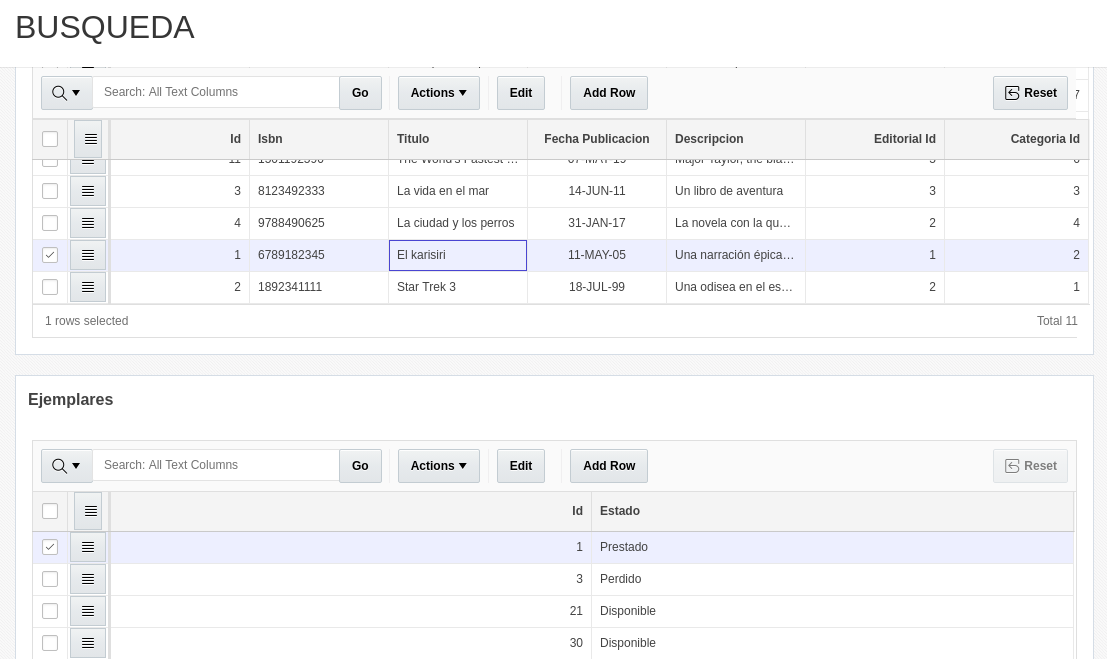
\includegraphics[width=0.95\textwidth]{biblio-busqueda_ejemplares}
  \caption{Búsqueda de ejemplares}
  \label{fig:biblio-busqueda_ejemplares}
\end{figure}